\clearpage

\lehead[]{\sf\hspace*{-2.00cm}\textcolor{white}{\colorbox{lightblue}{\parbox[c][0.70cm][b]{1.60cm}{
\makebox[1.60cm][r]{\thechapter}\\ \makebox[1.60cm][r]{ÜBUNG}}}}\hspace{0.17cm}\textcolor{lightblue}{\chaptertitle}}
\rohead[]{\textcolor{lightblue}{\chaptertitle}\sf\hspace*{0.17cm}\textcolor{white}{\colorbox{lightblue}{\parbox[c][0.70cm][b]{1.60cm}{\thechapter\\
ÜBUNG}}}\hspace{-2.00cm}}
%\chead[]{}
\rehead[]{\textcolor{lightblue}{AvHG, Inf, My}}
\lohead[]{\textcolor{lightblue}{AvHG, Inf, My}}

\section{Einfache Dialogelemente -- Übungen}

\subsection{Aufgabe 1: Layout-Manager austesten}

Teste die beiden wichtigsten Layout-Manager und das NULL-Layout aus, in dem du
jeweils eine Anwendung erzeugst, die fünf verschiedene Buttons (mit den
Aufschriften \myUserInput{A}, \myUserInput{B}, \myUserInput{C},
\myUserInput{D} und \myUserInput{E}) mit dem jeweiligen Layout-Manager
anordnet. Beim Klick auf die Buttons soll in dieser einfachen Vorübung noch
nichts geschehen.

\begin{compactenum}[a)]
\item \myClass{FlowLayout}
\item \myClass{GridLayout} mit zwei Zeilen und drei Spalten
\item NULL-Layout
\end{compactenum}


\subsection{Aufgabe 2: Knopfdrücke zählen}

Programmiere ein \myClass{JFrame} mit einem \myClass{JButton} und einem
\myClass{JLabel}. Gib im Label einen Text aus, der angibt, wie oft der Button
gedrückt wurde. Bei jedem Drücken des Buttons wird der Text angepasst. Verwende
dazu einen Layout-Manager. Ich empfehle das \myClass{FlowLayout}. Du darfst dich
aber auch für einen anderen Layout-Manager entscheiden (nicht NULL-Layout).

\vspace{3mm}

\begin{minipage}{0.75\textwidth}
\subsection{Aufgabe 3: Fahne im Wind}

\vspace{4mm}

Zeichne eine Fahne, die je nach Windrichtung nach rechts oder nach links
ausgerichtet ist. Die Windrichtung wird mit einer \myClass{JCheckBox}
ausgewählt. Wenn der Benutzer die Checkbox anklickt, dreht sich die Fahne sofort
in die neue Richtung. Damit die Fahne neu gezeichnet wird, muss im Frame die
Methode \lstinline|repaint()| aufgerufen werden.
\end{minipage}
\hfill
\begin{minipage}{0.25\textwidth}
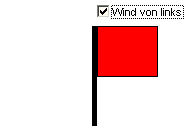
\includegraphics[width=1.0\textwidth]{./inf/SEKII/24_Java_GUI-Komponenten/FahneImWind.png}
\end{minipage}


\subsection{Aufgabe 4: Anrede}

Programmiere ein \myClass{JFrame}, das folgendes Aussehen hat:

\begin{center}
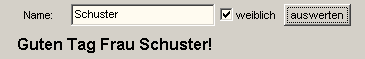
\includegraphics[width=0.6\textwidth]{./inf/SEKII/24_Java_GUI-Komponenten/Anrede.png}
\end{center}

Der Benutzer kann im Textfeld einen Namen eingeben. Wenn man auf den Button
drückt, wird der Benutzer höflich begrüßt. Dabei wird die Checkbox ausgewertet,
um zu erkunden, ob der Benutzer mit „Frau“ oder mit „Herr“ angeredet werden
soll. Wenn der Benutzer zum Beispiel den Namen „Meyer“ eingegeben hat und die
Checkbox nicht selektiert ist, wird ausgegeben: „Guten Tag Herr Meyer!“.


\subsection{Aufgabe 5: RGB-Farben mischen}

Programmiere ein \myClass{JFrame}, in dem man die RGB-Werte als Zahlen eingeben
kann. Wenn man auf einen Button drückt wird mit den eingegebenen RGB-Werten ein
Objekt der Klasse \myClass{Color} erzeugt. Im Konstruktor der Klasse
\myClass{Color} werden als Parameter die drei Farbwerte übergeben. Anschließend
wird die Hintergrundfarbe des \myClass{JFrame}-Fensters und der
\myClass{JLabel}-Komponenten auf den gemischten Farbwert gesetzt.

\begin{minipage}{0.5\textwidth}
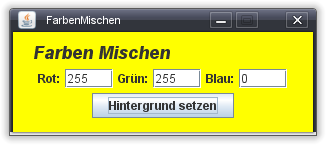
\includegraphics[width=1.0\textwidth]{./inf/SEKII/24_Java_GUI-Komponenten/FarbenMischen.png}
\end{minipage}
\hfill
\begin{minipage}{0.4\textwidth}
\subsubsection{Konvertierung von \myClass{String} nach \myClass{int}}

Beispiel:

\begin{lstlisting}
String text = "77";
int zahl = Integer.parseInt(text);
\end{lstlisting}
\end{minipage}